\documentclass{beamer}
\usetheme{Madrid}
\usepackage[normalem]{ulem}
\usepackage{attrib}

\begin{document}

\title{Team D Project Plan}
\author[CK, TW, ES, AM, JW, \& FS]{Cory Kolbeck, Tony Wooster, Erik Swanson, Adrian Miranda, Justin Wagner, and Federico Saldarini}
\institute[PSU]{
  Portland State University\\
  Department of Computer Science\\
  Portland, Oregon\\
}

\begin{frame}
  \titlepage
\end{frame}

\begin{frame}{Overview and Deliverables}
  \begin{center}{
      \large
      \textbf{We are to implement client libraries to provide asynchronous communication with a Burrow message queue server.}

      \vspace{1cm}
      
      The code for these libraries will reside on Github, and the sponsor will link to them from the main Burrow site. 
      Documentation will reside on the main Burrow website. 
    }
  \end{center}
\end{frame}

\begin{frame}{What is Burrow?}
  \begin{quote}
    "Burrow is a message queue that can be used in a variety of environments, from simple in-process queues to multi-tenant cloud services. The design is extremely modular and can be configured or extended to accommodate many use cases."
  \end{quote}\attrib{burrow.openstack.org}
\end{frame}

\begin{frame}{Assumptions}

  \begin{itemize}
  \item The code will be maintained by the OpenStack community
  \item The code will continue to reside on Github, or possibly be moved to launchpad
  \item Documentation will be pushed to Burrow's launchpad \texttt{bzr} repo, and hosted on burrow.openstack.org
  \item Authentication is outside the scope of this project
  \end{itemize}

\end{frame}

\begin{frame}{Restraints}

  \begin{itemize}
  \item Project will be distributed under the Apache2 license, and any libraries used must be compatible.
  \item All calls in to our library must be nonblocking.
  \item Maven will be used for Java builds.
  \item The Pandora autoconf macro set will be used for C builds.
  \item Minimal dependence on external libraries.
  \end{itemize}

\end{frame}

\begin{frame}{Plan Overview}
  The team will be split into two teams of three.
  Erik, Justin, and Cory will create a library in Java.
  Tony, Fede and Adrian will create a library in C.

  \begin{enumerate}
  \item \sout{Meet with Eric Day to discuss project details}
  \item \sout{Decide on target languages}
  \item \sout{Create skeleton projects and set up burrow continuous integration infrastructure}
  \item Research asynchronous I/O
  \item Create blocking memory backends
  \item Research and choose JSON and HTTP libraries
  \item Create blocking http backend 
  \item \sout{Choose language appropriate callback mechanisms}
  \item Write asynchronous memory backend
  \item Write asynchronous http backend
  \item Write functional tests
  \item \textit{Time Allowing} Write small projects which use our libraries in interesting ways.
  \end{enumerate}
\end{frame}

\begin{frame}{C Gantt Chart}
  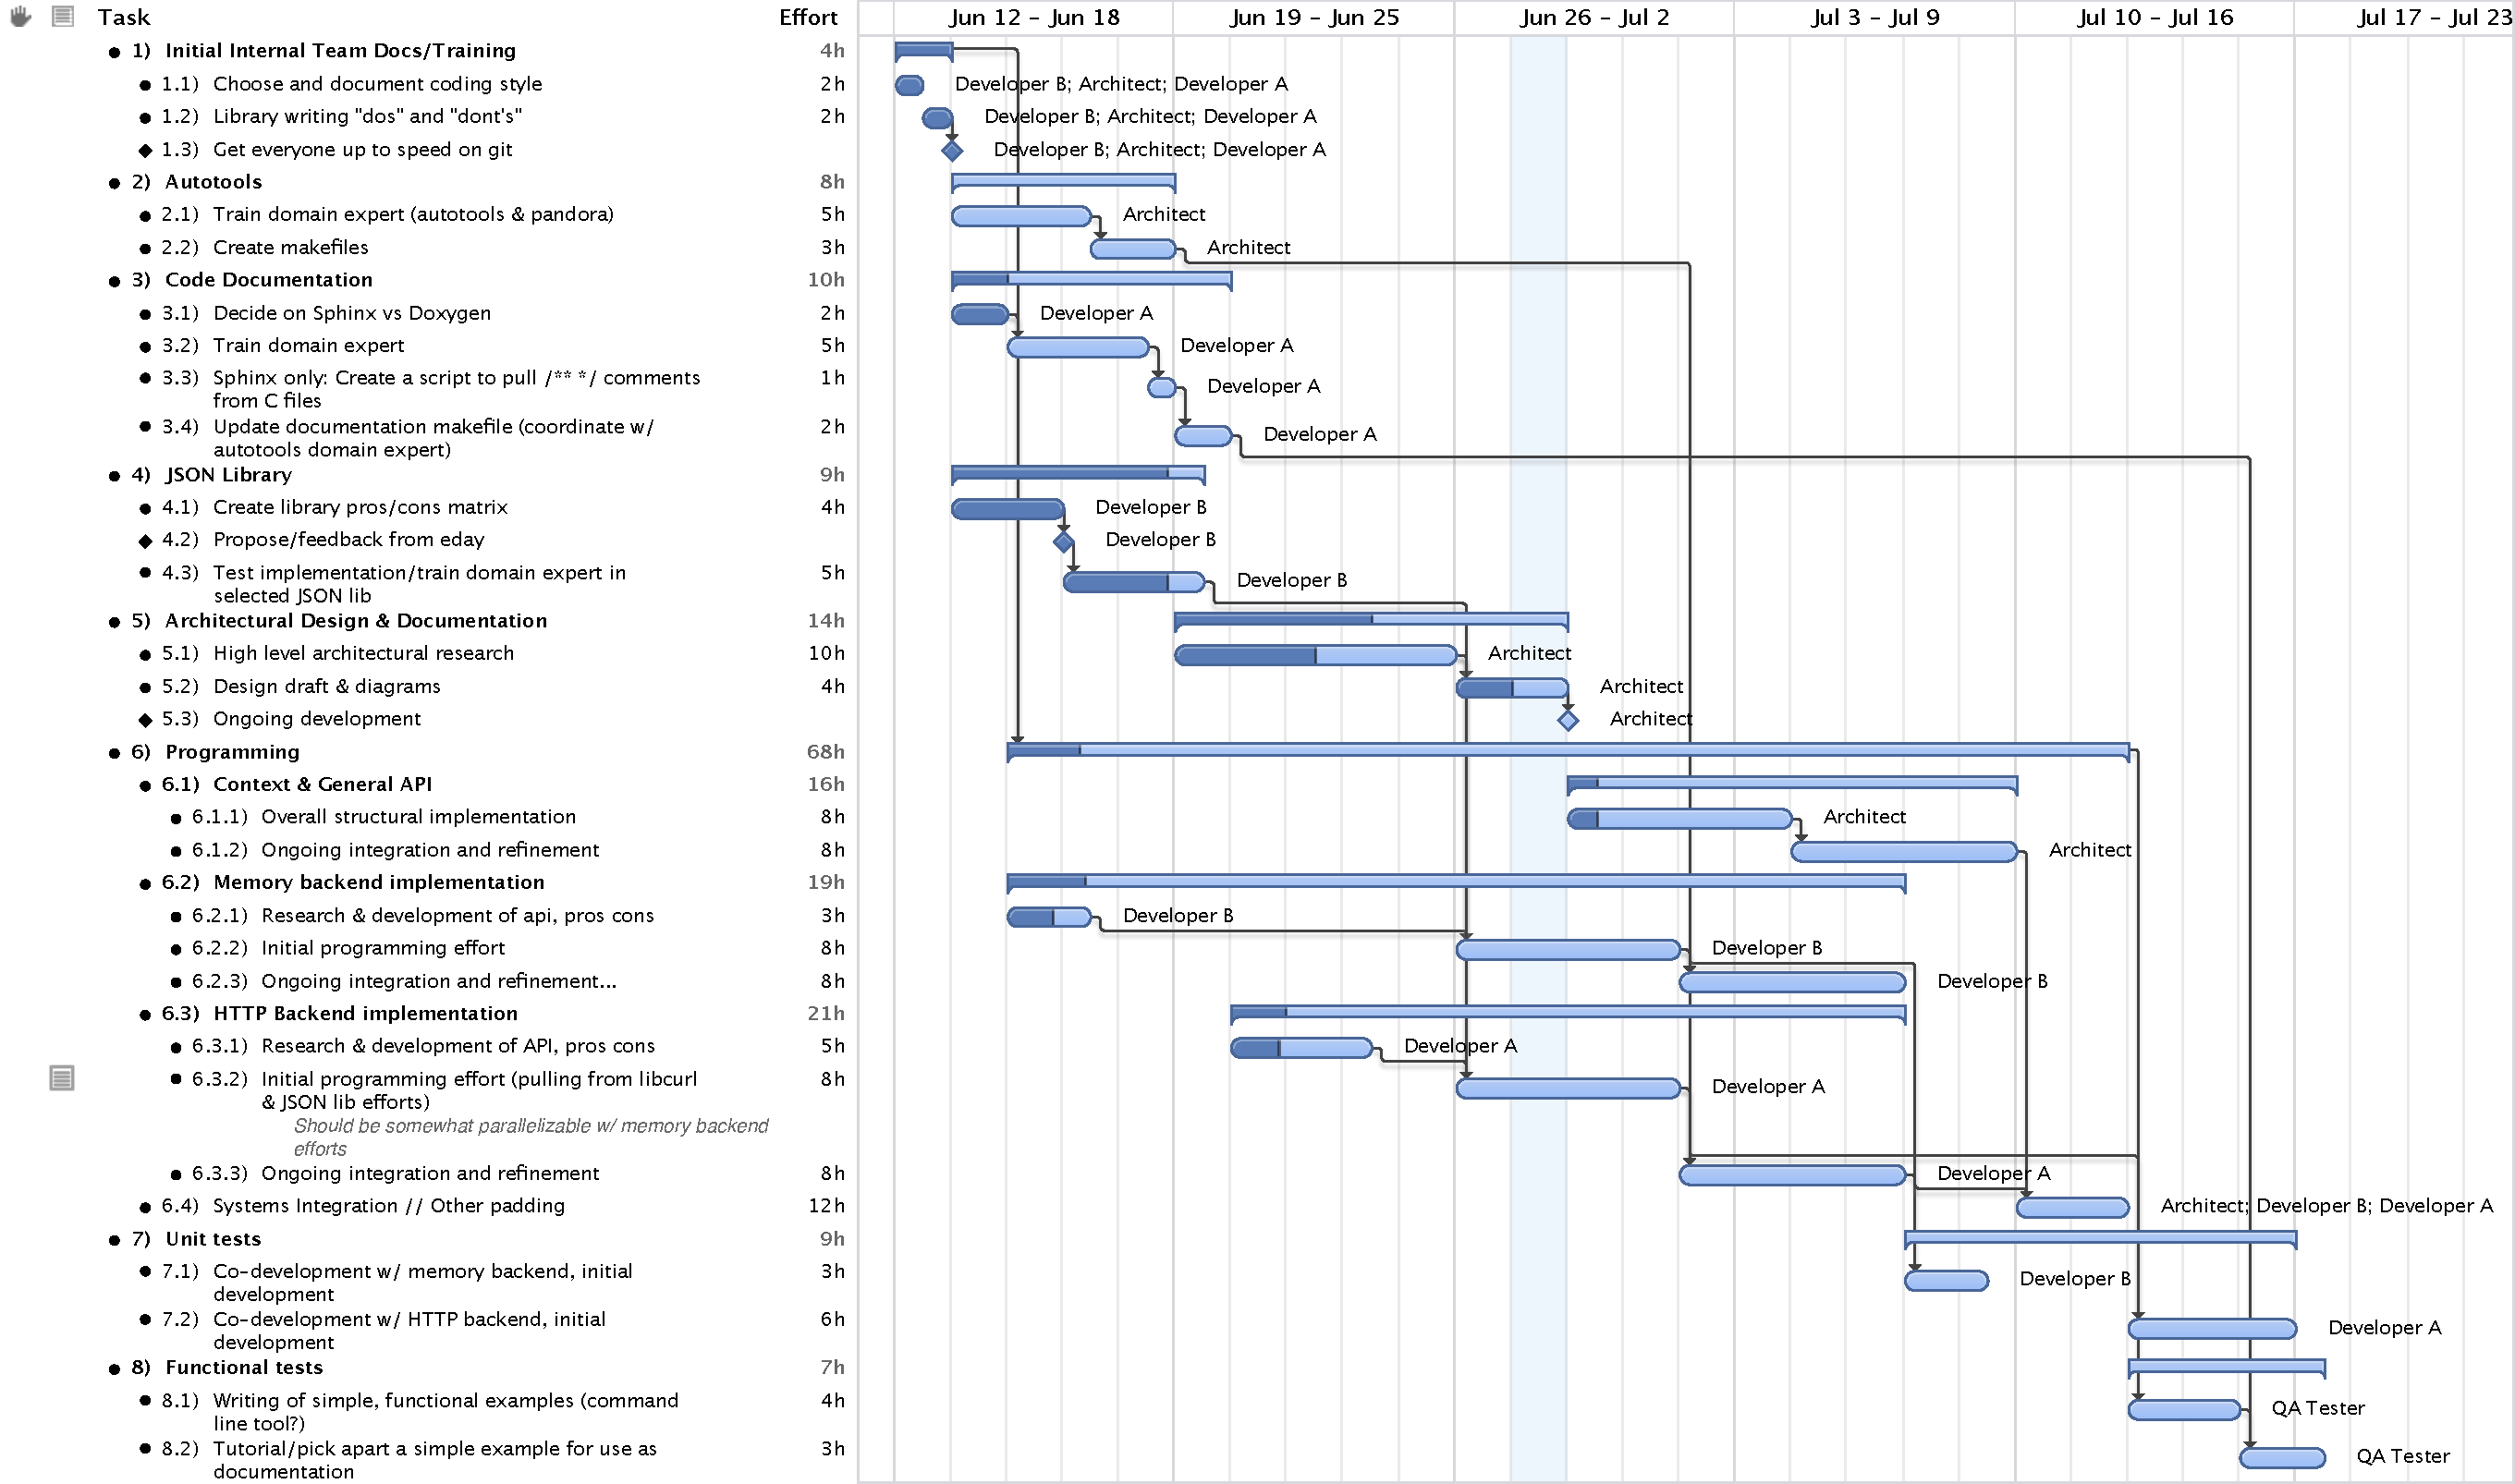
\includegraphics[width=0.95\linewidth]{C-Gantt.pdf}
\end{frame}

\begin{frame}{Java Gantt Chart}
  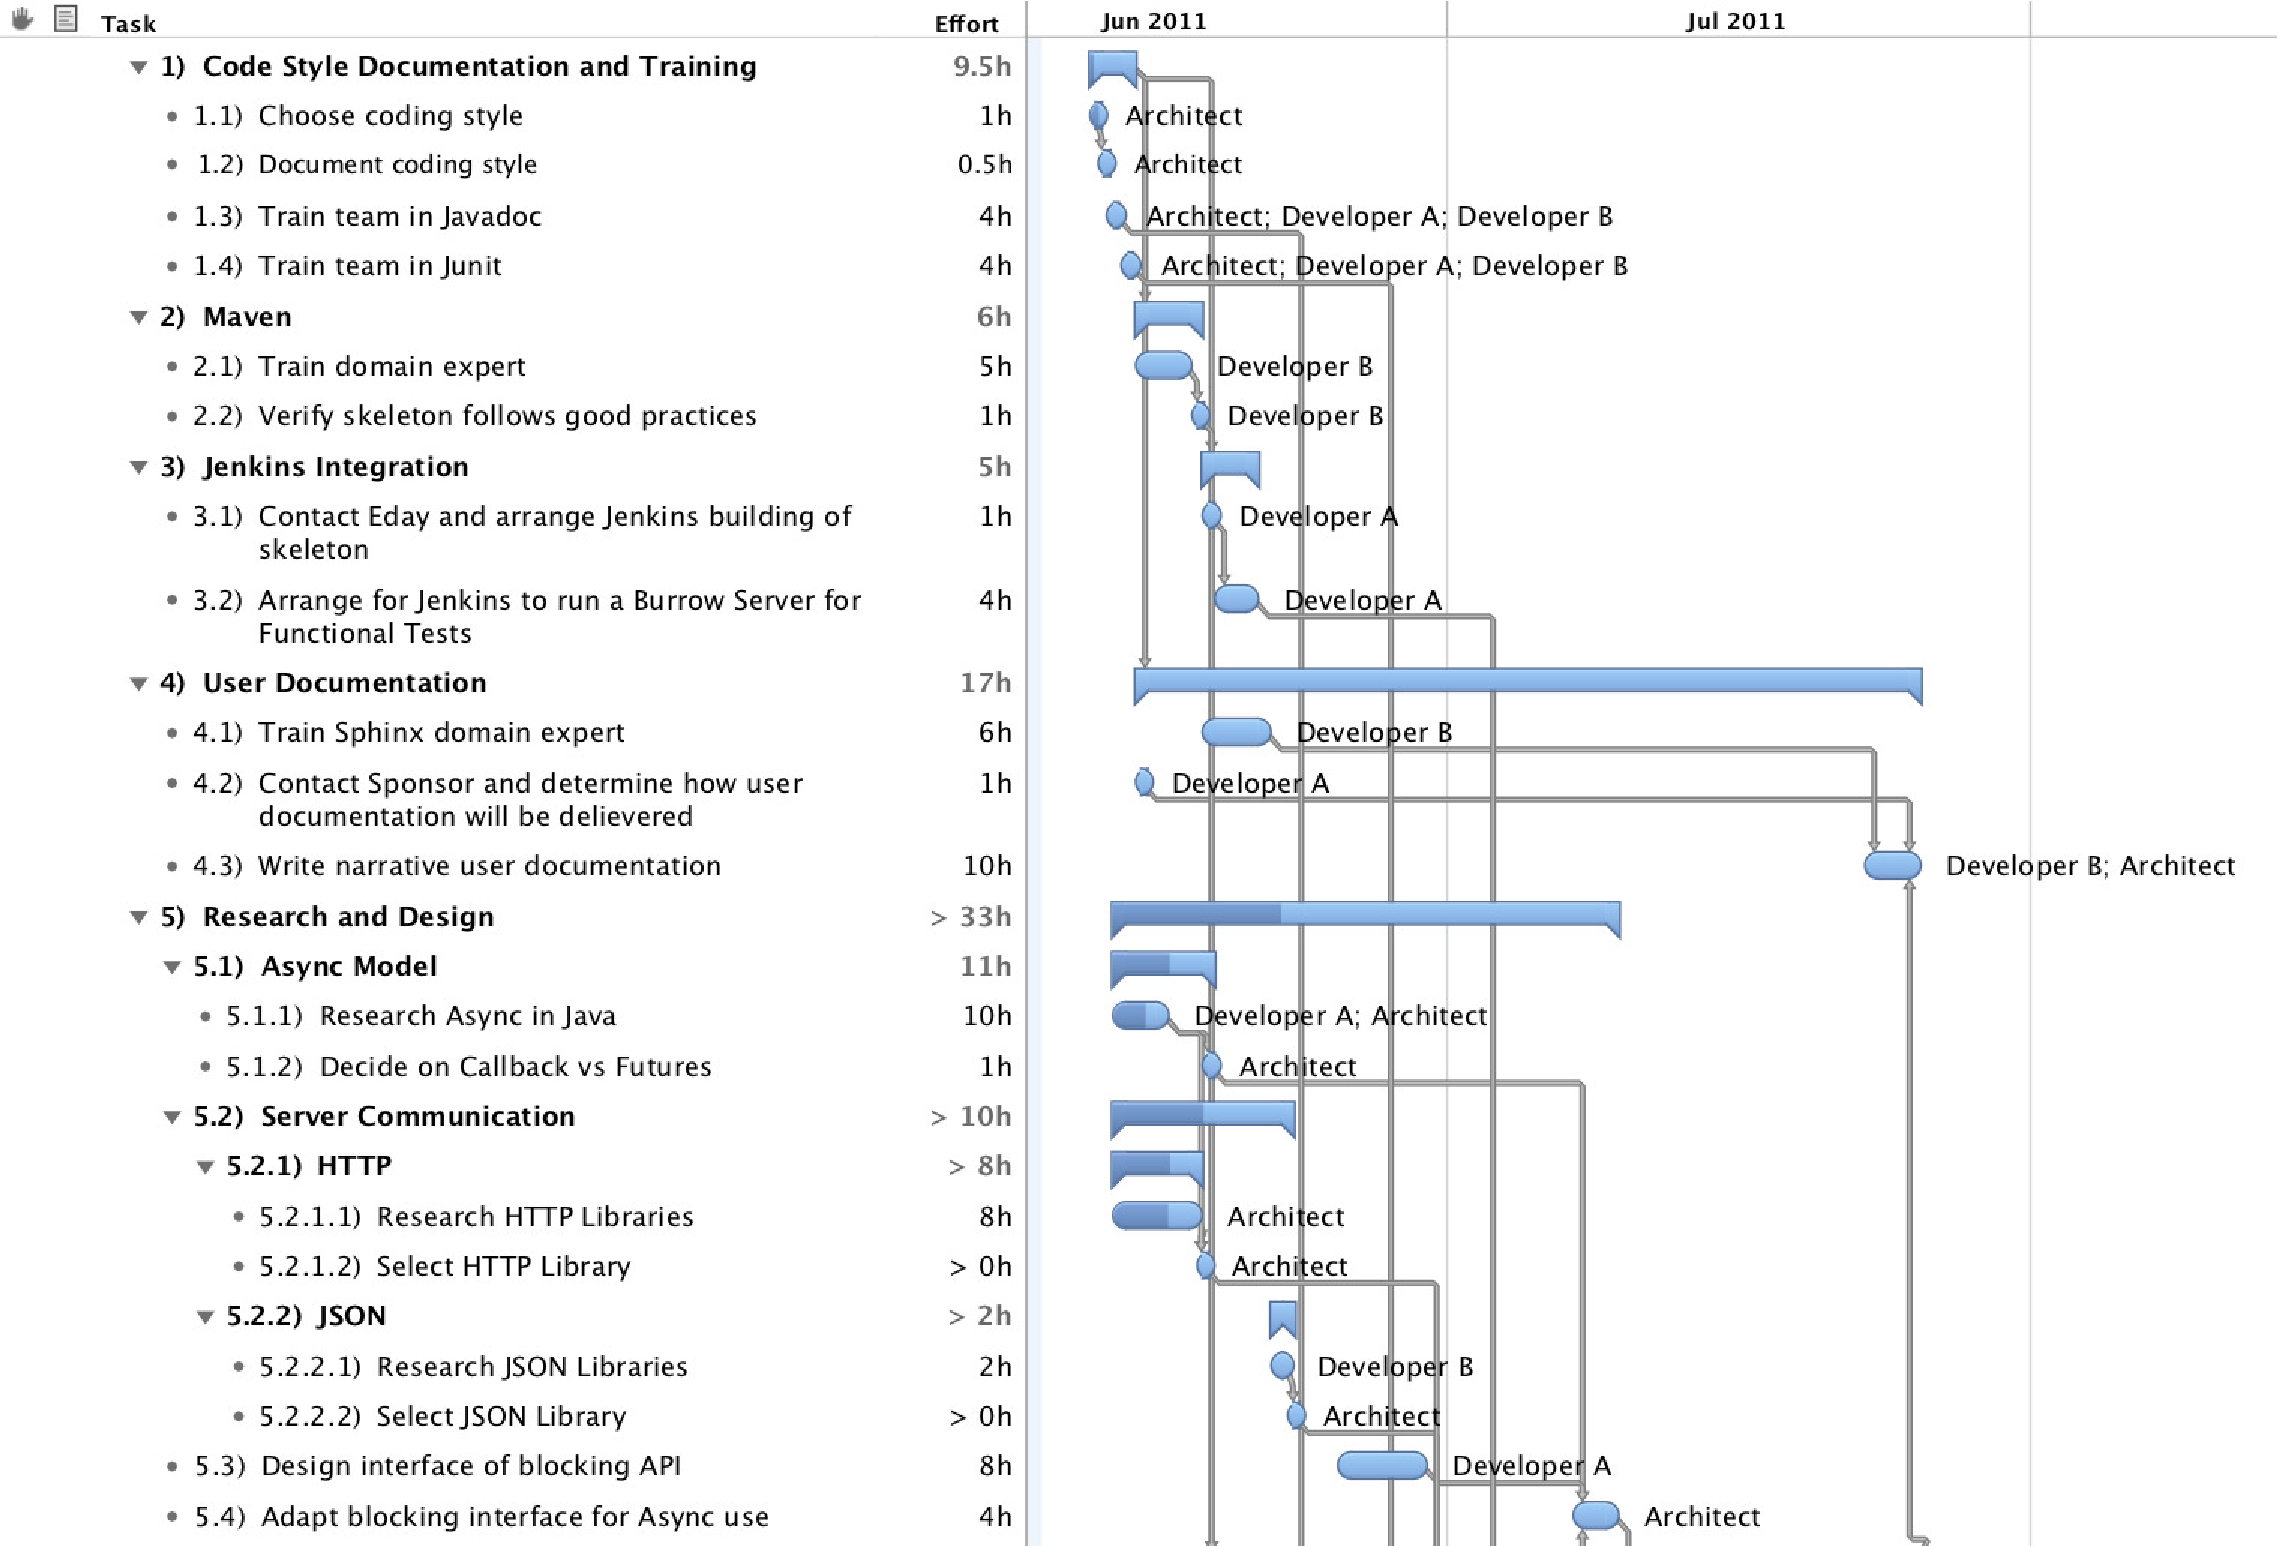
\includegraphics[width=0.95\linewidth]{Java-Gantt-P1.pdf}
\end{frame}

\begin{frame}{Java Gantt Chart}
  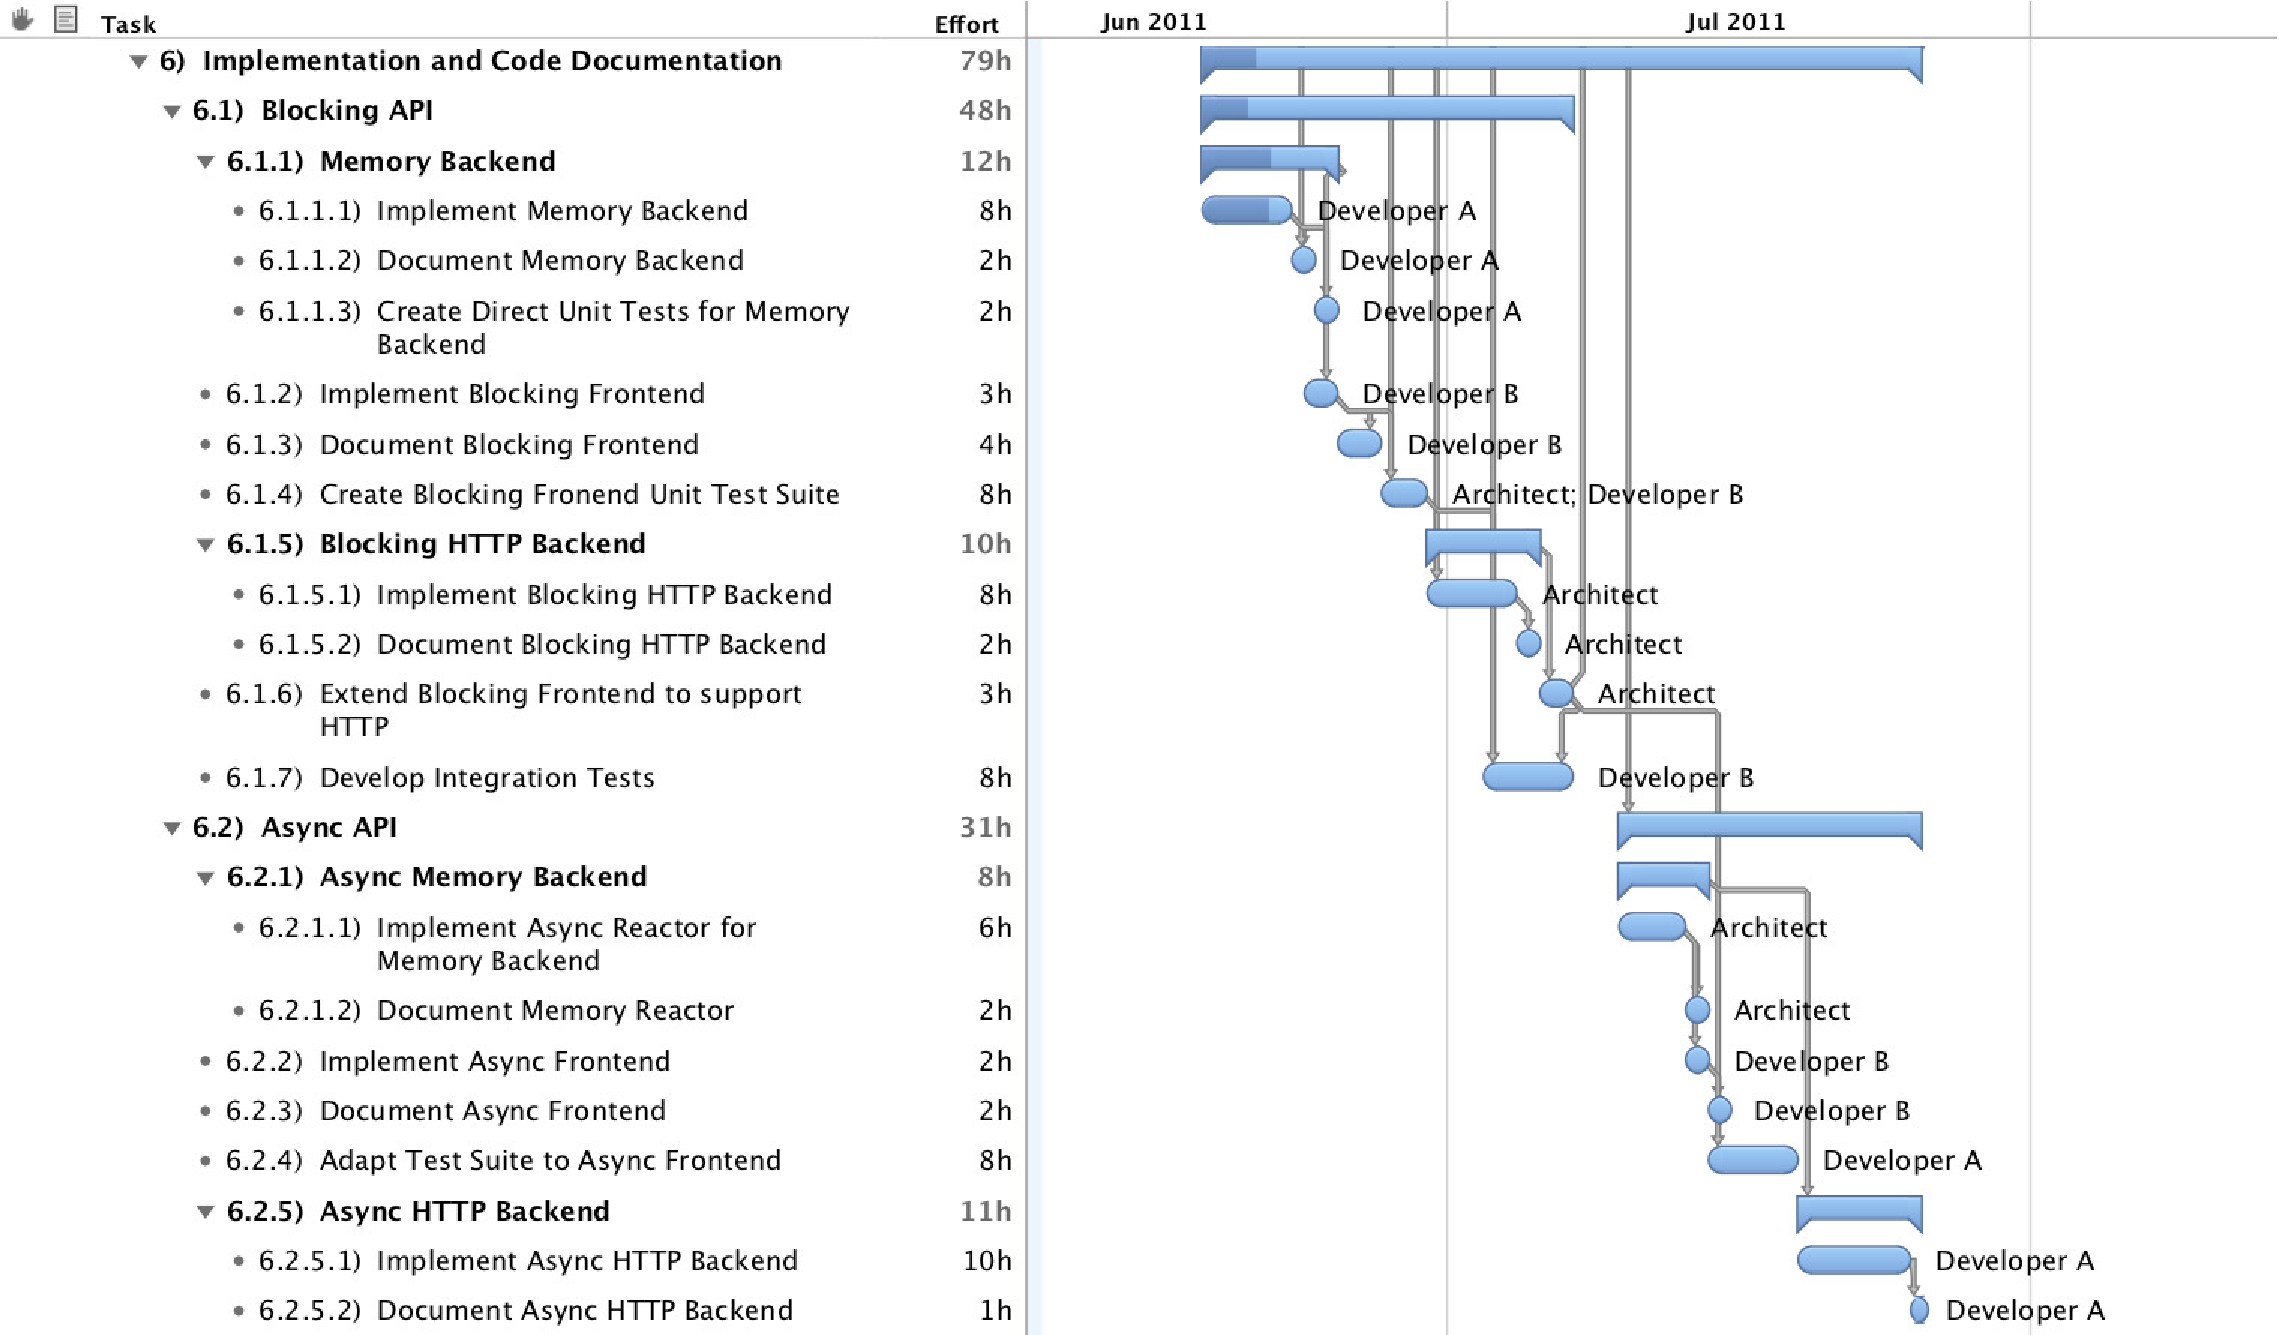
\includegraphics[width=0.95\linewidth]{Java-Gantt-P2.pdf}
\end{frame}

\begin{frame}{C Milestones}
  \begin{center}{\small
    \begin{tabular}{| c | p{10cm} |}
      \hline
      \emph{Week of} & \emph{Deliverable}\\ \hline \hline
      Jun 05 & Pert Chart, Architecture Overview, Use of Jenkins CI \\ \hline
      Jun 12 & Arch Discussed/Approved w/ Sponsor, Support Libs, Docs, Source Style chosen\\ \hline
      Jun 19 & -\\ \hline
      Jun 26 & Simplified Async HTTP and  Memory Backend implemented; Architecture largely documented\\ \hline
      Jul 03 & HTTP \& Memory Component Implementation, First Long-Term Unit Tests\\ \hline
      Jul 10 & Development \& Testing Continues -- First True Functional Tests / Demo Programs\\ \hline
      Jul 17 & Feature Complete w/ Bugs \& Testing Gaps, Docbook Begins\\ \hline
      Jul 24 & .. slack ..\\ \hline
      Jul 31 & Feature Complete w/ 70\% test coverage, finalization: Project Closing \& Deliverables\\\hline
      Aug 08 & Final Presentation\\ \hline
    \end{tabular}
    }
  \end{center}
\end{frame}

\begin{frame}{Java Milestones}
  \begin{center}
    \begin{tabular}{| c | l |}
      \hline
      \emph{Week of} & \emph{Deliverable}\\ \hline \hline
      Jun 05 & Pert Chart, Architecture Overview, Use of Jenkins CI \\ \hline
      Jun 12 & -\\ \hline
      Jun 19 & -\\ \hline
      Jun 26 & Blocking Memory Backend\\ \hline
      Jul 03 & Blocking HTTP Backend\\ \hline
      Jul 10 & -\\ \hline
      Jul 17 & Async Memory Backend\\ \hline
      Jul 24 & Async HTTP Backend\\ \hline
      Jul 31 & Narrative Documentation, Sponsor Delivery\\\hline
      Aug 08 & Final Presentation\\ \hline
    \end{tabular}
    \end{center}
\end{frame}

\begin{frame}{Meetings and Reviews}
  \begin{itemize}
  \item In person meetings with sponsor every 1-2 weeks.
  \item IRC consultation as needed.
  \item Reviews at milestones as previously noted.
  \end{itemize}
\end{frame}

\begin{frame}{Resource Identification}
  \begin{center}
    \begin{tabular}{|c|c|}
      \hline
      \emph{Name} & \emph{Available Hours/Week}\\ \hline \hline
      Justin & 8-10\\ \hline
      Adrian & 8-10\\ \hline
      Tony & 10+\\ \hline
      Erik & 10-15\\ \hline
      Federico & 10+\\ \hline
      Cory & 10-15 \\
      \hline
    \end{tabular}
  \end{center}
\end{frame}

\begin{frame}{Configuration Management}
  \begin{itemize}
  \item Github will be used for source control
  \item Ticketing and bug reporting will be through Github's builtin utilities
  \item Should it become necessary, language leads will be in charge of resolving merge conflicts
  \item Unit testing and code coverage reports will be through the Jenkins continuous integration framework.
  \end{itemize}
\end{frame}

\begin{frame}{Roles}
  \begin{center}
    {\footnotesize
      \begin{tabular*}{.966\linewidth}{| r | p{7.7cm} | l |}
        \hline
        \emph{Role} & \emph{Responsibility} & Initial\\ \hline \hline
        Manager & Coordinate general geetings and maintain schedules & C\\ \hline
        POC & Maintain communication between team and sponsor & C\\ \hline
        Integration & Support Jenkins and Github issues & C\\ \hline 
        Java Lead & Architect Java library and delegate coding and research tasks & E\\ \hline
        C Lead & Architect C library and delegate coding and research tasks & T\\ \hline
        Java Dev & Implement designs of Java lead & CJE\\ \hline
        C Dev & Implement designs of C lead & AFT\\ \hline
        Support & Maintain Shared Machines & C\\ \hline
        Unit Testing & Code unit tests for every function & All\\ \hline
        Func. Testing & Create functional tests for each language & tbd \\ \hline
        API Docs & Write language specific documentation & tbd \\ \hline
        General Docs & Create a language agnostic guide to coding burrow clients & T\\ \hline
    \end{tabular*}
    }
  \end{center}
\end{frame}

\begin{frame}{Risk Management}
  \begin{itemize}
  \item Risk: Team member drops out\\
    Consequence: Fewer man-hours available\\
    Mitigation: Scheduling a week of slack time
  \item Risk: Architect drops out\\
    Consequence: Possible loss of grand plan\\
    Mitigation: Documentation, regular meetings to keep team members in the loop
  \item Risk: Sponsor pulls out/disappears\\
    Consequence: Main link to Burrow project severed, loss of technical guidance\\
    Mitigation: Forming a relationship with other members of the OpenStack community working on Burrow
    

  \end{itemize}
\end{frame}

\begin{frame}{QA and Deployment}
  \begin{itemize}
  \item Unit and regression testing will be ongoing using Burrow's existing Jenkins continuous integration system.
  \item Functional testing will take place in the weeks leading up to code freeze.
  \item Deployment will consist of linking to our existing Github repositories (or possibly official forks)
    from burrow.openstack.org.
  \item Documentation will be pushed to the Burrow \texttt{bzr} for inclusion in the Burrow wiki.
  \end{itemize}
\end{frame}

\end{document}
